\documentclass[conference]{IEEEtran}
\IEEEoverridecommandlockouts

\usepackage{cite}
\usepackage{amsmath,amssymb,amsfonts}
\usepackage{algorithmic}
\usepackage{graphicx}
\usepackage{textcomp}
\usepackage{xcolor}
\usepackage{booktabs} % For nice tables
\usepackage[hidelinks]{hyperref} % <--- FÜGE DIESE ZEILE HINZU
\def\BibTeX{{\rm B\kern-.05em{\sc i\kern-.025em b}\kern-.08em
    T\kern-.1667em\lower.7ex\hbox{E}\kern-.125emX}}


\begin{document}

\title{Photosynthesis - Mechanisms}

\author{\IEEEauthorblockN{Luka Tadic}
\IEEEauthorblockA{\textit{Electrical Energy Systems and Electromobility (M.Sc.)} \\
\textit{Technische Hochschule Ulm (THU)}\\
Ulm, Germany \\
tadilu01@thu.de} 
}

\maketitle

\begin{abstract}
This paper explores how natural photosynthesis works, explaining its complex biological mechanisms in simple engineering and technical terms. As global energy demands increase, we need better ways to harvest and store solar energy. Plants have already solved this problem. In this paper, we look at the plant leaf not as a biological organism, but as a technical system: the cellular membrane acts as a solar panel, the electron transport chain works like an electrical circuit, and enzymes act as mechanical motors and chemical factories. By understanding these steps step-by-step, including their process efficiencies and limits, we can learn how to build artificial systems. Finally, the paper discusses how these biological blueprints are currently used to build artificial leaves (photoelectrochemical cells) that produce green hydrogen for the future energy grid.
\end{abstract}

\begin{IEEEkeywords}
Photosynthesis, Electron Transport, Bio-inspired Engineering, Energy Conversion, Artificial Leaf
\end{IEEEkeywords}

\section{Introduction}
One of the greatest challenges of our time is finding sustainable ways to generate and store energy. Modern technologies, like silicon solar panels, are very good at turning sunlight into electricity. However, electricity is hard to store in large quantities over long periods. Batteries are expensive and require rare materials \cite{lewisCosteffectiveSolarEnergy2007}. 

Nature, on the other hand, solved this problem billions of years ago. Through photosynthesis, plants capture sunlight and use that energy to build stable, energy-rich chemical compounds (sugars), which can be stored indefinitely. From an engineering perspective, a leaf is essentially a self-repairing, highly efficient biological factory. It absorbs solar photons, separates positive and negative electrical charges, and uses those charges to drive chemical manufacturing \cite{barberPhotosyntheticEnergyConversion2009}.

To truly understand how we can replicate this in technology, we must first understand how it works in nature. This paper translates the biology of photosynthesis into the language of engineering. We will break down the process into easy-to-understand technical components: light absorbers, electrical circuits, mechanical motors, and catalytic reactors. By the end of this paper, the reader will understand both the mechanisms of natural photosynthesis and how these principles are applied to build artificial devices that generate clean fuels, such as green hydrogen.

\section{Principles of Light Harvesting}
\subsection{The Membrane as a Solar Module}
The first step of energy conversion happens inside the plant's cells, specifically in a structure called the chloroplast. Inside the chloroplast, there are thin, flat membranes called thylakoid membranes. You can think of the thylakoid membrane as a biological solar panel or a p-n junction in a semiconductor \cite{gustSolarFuelsArtificial2009}. It acts as an electrical insulator—a barrier separating the inside from the outside. Because it is an insulator, it allows the plant to build up an electrical voltage and a concentration difference across it, which is the foundation of storing energy.

\subsection{Catching the Sun: Antenna Complexes}
A technical solar module needs a large surface area to catch sunlight. Plants use networks of proteins and green pigments (like chlorophyll), which are called Light-Harvesting Complexes (LHC) \cite{scholesLessonsNatureSolar2011}. Instead of giving every single "chemical reactor" its own direct light source, the LHC acts like a large satellite dish or a funnel. 

When a particle of light (a photon) hits a pigment molecule in this outer dish, the molecule absorbs the energy. This creates an "exciton," which is simply an energized, excited state (similar to an electron-hole pair in a solar cell). Now, this energy needs to travel to the center of the system to be used. 

Instead of flowing like normal electrical current in a copper wire, this energy jumps from one pigment molecule to the next. This jumping process is called Förster Resonance Energy Transfer (FRET). FRET acts like a series of tuning forks passing a vibration along. The efficiency of this jump ($E_{FRET}$) depends strongly on the distance ($r$) between the molecules, as described by the following mathematical equation:

\begin{equation}
E_{FRET} = \frac{1}{1 + \left(\frac{r}{R_0}\right)^6}
\label{eq:fret}
\end{equation}

Here, $R_0$ is a specific distance where the transfer is exactly 50\% efficient. Because the plant's pigments are packed so closely and ordered perfectly, the energy funnels into the reaction center with an efficiency close to 100\% \cite{flemingPrimaryStepsPhotosynthesis1994}. Almost no light energy is lost in this initial step.

% --- BILD 1 ---
\begin{figure*}[htbp]
    \centering
    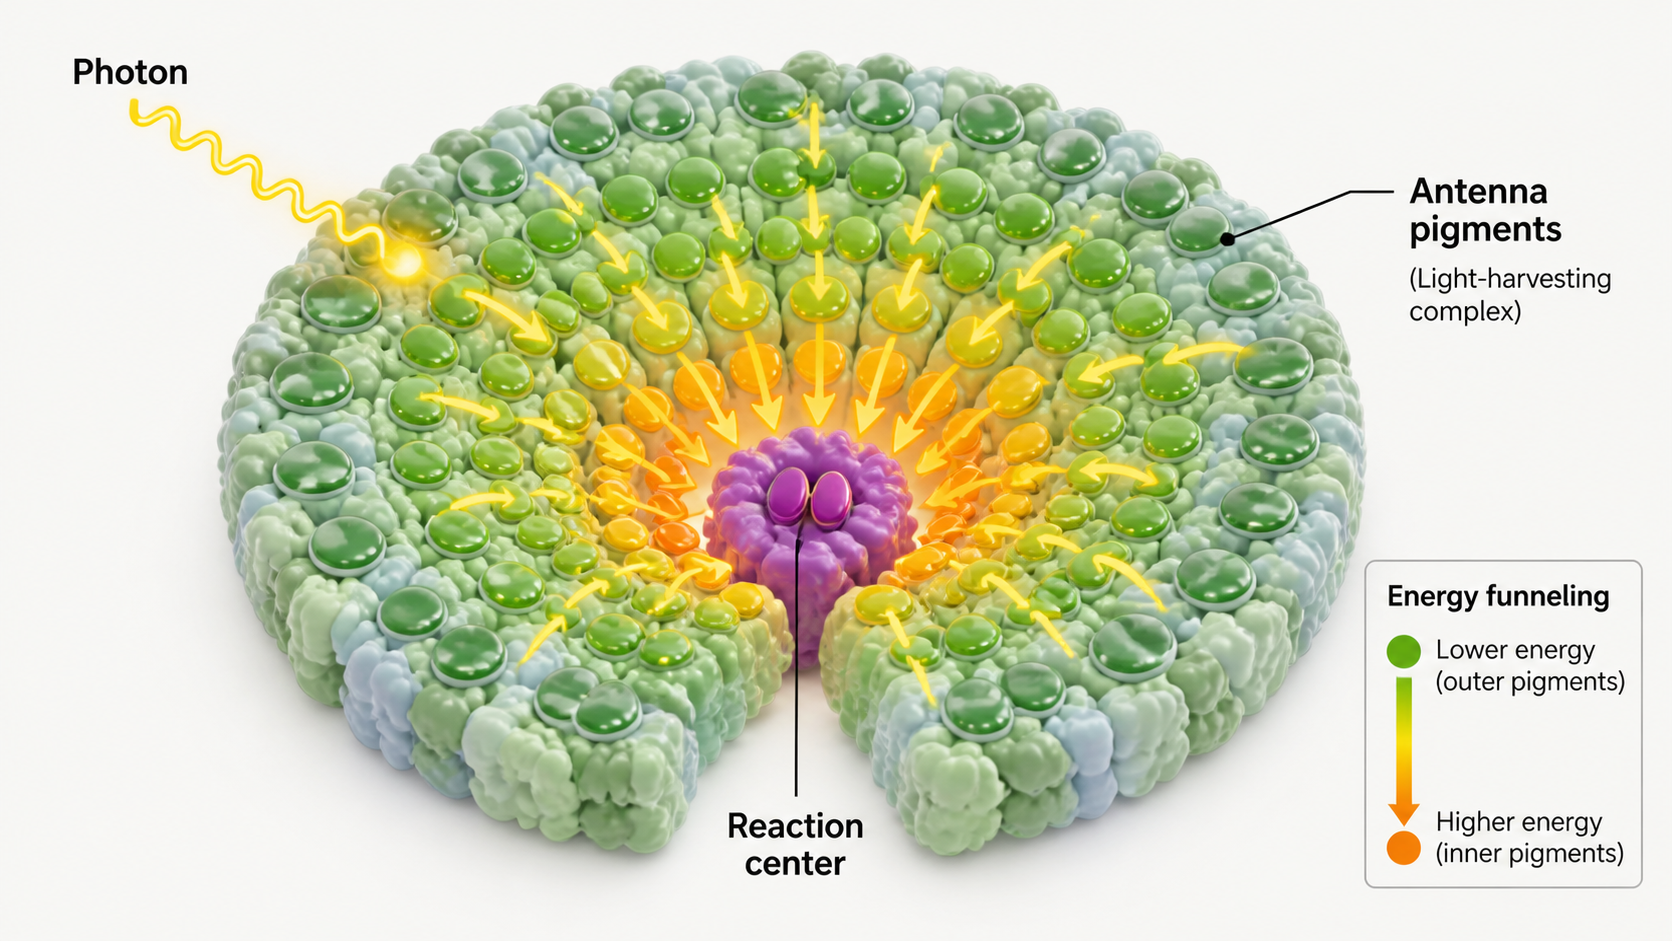
\includegraphics[width=0.7\textwidth]{images/funnel.png} 
    \vspace{0.2cm}
    \caption{The funnel model of light harvesting. Energy from incoming photons is guided via highly efficient Förster Resonance Energy Transfer (FRET) through a gradient toward the reaction center. Image generated using Perplexity AI.}
    \label{fig:antenna}
\end{figure*}

\section{The Biological Electrical Circuit}
Once the light energy reaches the center (the reaction center), the system converts the excited energy into actual moving electrons. From this point on, we can look at the process as a biological direct current (DC) circuit featuring pumps, wires, and power supplies.

\subsection{Photosystem II: Splitting Water}
The starting point of this circuit is a component called Photosystem II (PSII). The energy delivered by the light funnel causes the core of PSII to eject an electron. Because it lost an electron, PSII becomes "hungry" for a replacement, developing a very strong electrical pull (a redox potential of roughly +1.2 Volts) \cite{barberPhotosyntheticEnergyConversion2009}. 

This voltage is strong enough to perform a remarkable feat: it rips water ($H_2O$) molecules apart to steal their electrons. This process is called photolysis. The overall chemical equation for this biological water splitting is:

\begin{equation}
2H_2O \xrightarrow{\text{light}} O_2 + 4H^+ + 4e^-
\label{eq:water_oxidation}
\end{equation}

For every two water molecules split, the system gets four electrons ($e^-$) to power the circuit, leaves behind four protons ($H^+$), and releases oxygen ($O_2$) as "waste" into the air \cite{mcevoyWatersplittingChemistryPhotosystem2006}. Technically, PSII is a perfectly functioning, solar-powered water electrolyzer.

This overall reaction looks simple on paper, but it presents a massive technical challenge. Stripping four electrons from two water molecules simultaneously requires overcoming a massive energetic barrier, while doing it sequentially would create highly reactive and destructive intermediate oxygen species (like hydrogen peroxide) that destroy the cell. 

Nature solves this thermodynamic problem using a component called the Oxygen-Evolving Complex (OEC), which acts as a catalytic charge accumulator. Described biologically by the "Kok cycle," the OEC features a cluster of manganese and calcium atoms that can cycle through five different oxidation states ($S_0$ to $S_4$). Like a biological capacitor, it stores the positive charges from four successive photon-driven electron ejections before discharging them all at once to split the water molecule efficiently and safely \cite{mcevoyWatersplittingChemistryPhotosystem2006}. Replicating this exact four-electron synchronized transfer remains one of the hardest challenges in designing artificial water-splitting catalysts today.

% --- BILD 2 (ZWEISPALTIG) ---
\begin{figure*}[htbp]
    \centering
    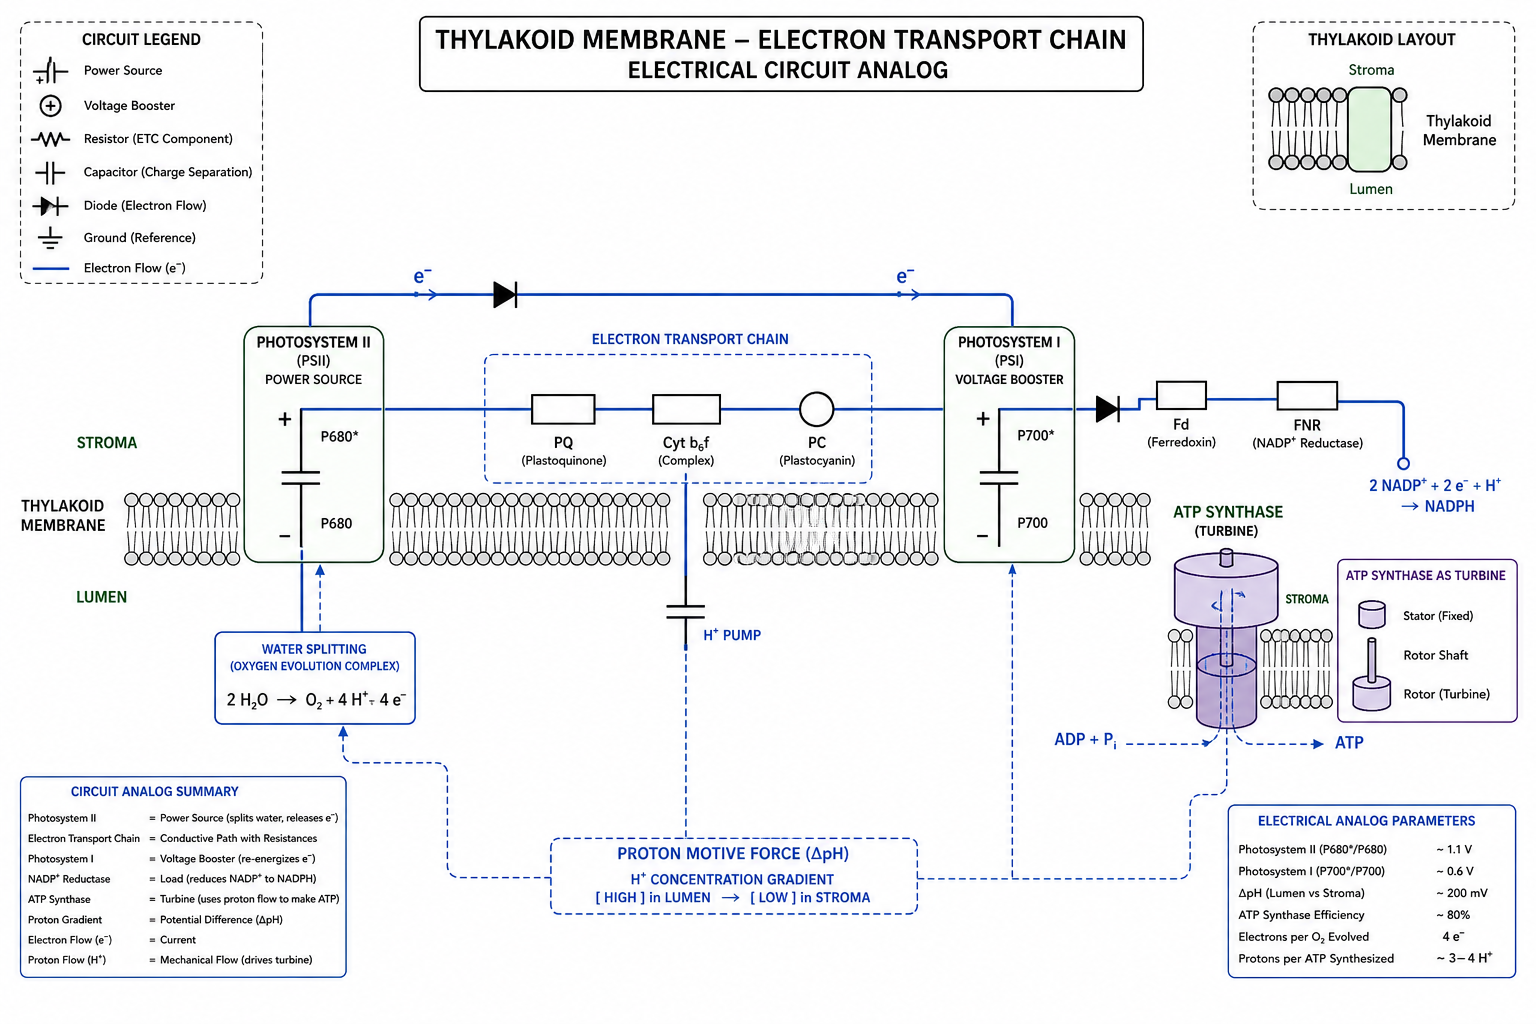
\includegraphics[width=0.95\textwidth]{images/circuit.png} 
    \vspace{0.2cm}
    \caption{The electron transport chain viewed as a biological circuit. Electrons flow from water to NADP+ via two solar-powered voltage boosts, while protons are pumped across the membrane to drive the ATP synthase motor. Image generated using ChatGPT AI.}
    \label{fig:circuit}
\end{figure*}
% --------------------------

\subsection{The "Wires" and the Second Voltage Boost}
The extracted electrons now flow through the membrane. They are carried by a molecule called plastoquinone, which acts like a mobile biological wire. The electrons flow to a middle station called the Cytochrome $b_6f$ complex. As the electricity flows through it, Cytochrome uses that power to pump even more protons ($H^+$) across the membrane \cite{cramerTransmembraneTrafficCytochrome2006}.

Because the electrons lose energy while powering the pump, they need a second boost. They arrive at Photosystem I (PSI), which absorbs another photon of light to re-energize the electrons. This pushes the electrons to a very high energy level so they can be stored in a chemical carrier molecule called NADPH \cite{nelsonStructureFunctionPhotosystems2006}. Because it requires two upward energy boosts, this whole mechanism is known to biologists as the "Z-scheme."

\subsection{ATP Synthase: A Biological Hydroelectric Dam}
By constantly pumping protons ($H^+$) across the biological membrane, the system builds up high pressure on one side—exactly like water building up behind a hydroelectric dam.

To relieve this pressure, the protons flow back across the membrane through a specialized enzyme called ATP Synthase. This enzyme is essentially a microscopic, mechanical rotary motor. As the protons flow through it, they push against a biological rotor, causing it to spin at thousands of revolutions per minute \cite{jungeATPSynthase2015}. This mechanical spinning forces two molecules (ADP and phosphate) together to create ATP, the universal energy battery of all living cells. Here, electrical pressure is converted into mechanical rotation, and finally into chemical energy.

\section{Process Efficiency and Carbon Fixation}
The light reactions provide temporary batteries (ATP and NADPH). However, the plant needs long-term storage, which is accomplished in the next stage.

\subsection{The Assembly Line: The Calvin Cycle}
To an engineer, the Calvin cycle is an isothermal (constant temperature), continuous-flow chemical reactor. It does not need light to function. Instead, it takes the ATP and NADPH batteries produced by the circuit and uses them as power to capture carbon dioxide ($CO_2$) from the air. It stitches the $CO_2$ together to build complex sugars \cite{bensonFollowingPathCarbon2002}. 

This process relies heavily on an enzyme called RuBisCO. While important, RuBisCO is famously slow and inefficient, sometimes grabbing oxygen by mistake instead of $CO_2$, which wastes energy \cite{anderssonCatalysisRegulationRubisco2008}. It is a slow assembly line, trading speed for the ability to build incredibly dense and stable fuel at normal outdoor temperatures.

\subsection{Calculating the Efficiency Limits}
In engineering, we measure how much input energy from the sun is actually converted into useful output energy. For standard silicon solar cells, physics dictates a hard theoretical limit called the Shockley-Queisser limit, which caps the maximum theoretical efficiency at about 33.7\% \cite{ruhleTabulatedValuesShockley2016}.

For natural photosynthesis, the overall energy efficiency ($\eta$) can be defined simply as:

\begin{equation}
\eta = \frac{\text{Energy Stored in Biomass}}{\text{Total Solar Energy Input}}
\label{eq:efficiency}
\end{equation}

While plants are extremely clever, their overall efficiency is surprisingly low. Plants only absorb a fraction of the color spectrum (reflecting green light), lose energy as heat, and consume energy just to keep their cells alive. Although the theoretical maximum biological efficiency is around 11\%, most plants in the real world only convert 1\% to 2\% of the sun's energy into stored biomass \cite{zhuImprovingPhotosyntheticEfficiency2010}.

% --- BILD-PLATZHALTER 3 (ZWEISPALTIG) ---
\begin{figure*}[htbp]
    \centering
    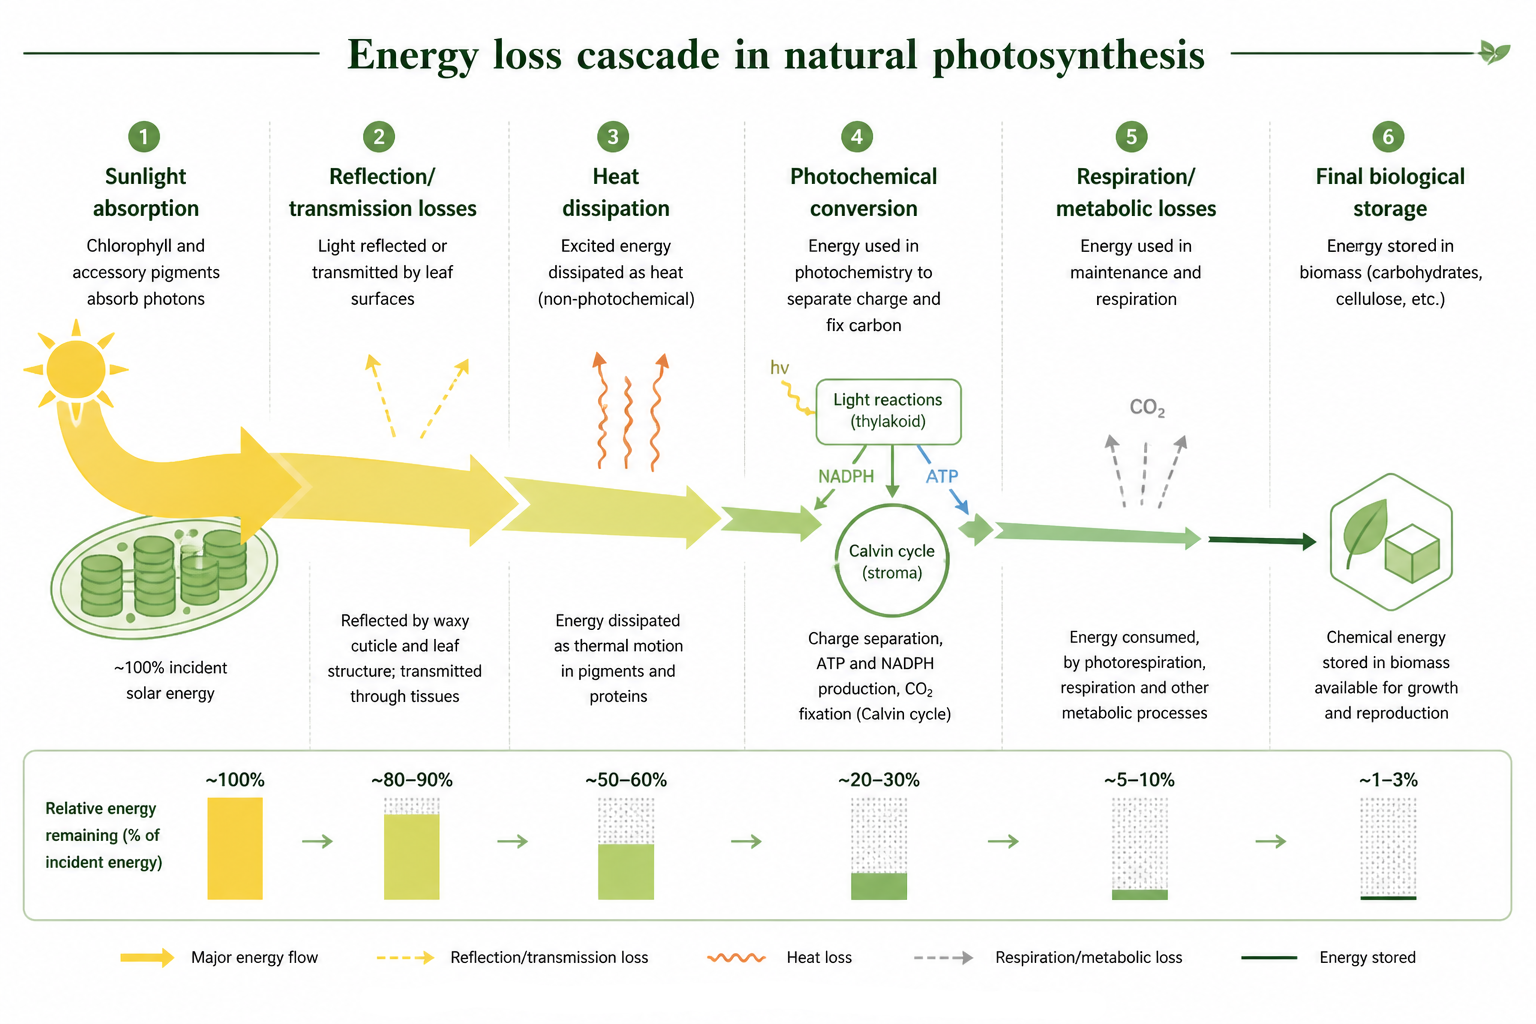
\includegraphics[width=0.9\textwidth]{images/efficiency.png}
    \vspace{0.2cm}
    \caption{Energy loss cascade in natural photosynthesis. Despite high efficiency in early light absorption, overall system losses reduce the final biological storage efficiency drastically. Image generated using Perplexity AI.}
    \label{fig:efficiency}
\end{figure*}
% --------------------------

\section{From Biology to Technology: Artificial Leaf Systems}
The ultimate goal of studying photosynthesis is not just to understand plants, but to copy their brilliant mechanisms while leaving behind their biological weaknesses (like the slow Calvin cycle and low efficiency). This field is called "Artificial Photosynthesis".

Instead of making sugar, the primary goal of engineers is to use sunlight and water to produce green hydrogen ($H_2$), a clean-burning fuel for the future.

\begin{table*}[htbp]
\caption{Systematic Comparison: Natural Photosynthesis vs. Artificial Photoelectrochemical Cells (PEC)}
\begin{center}
\renewcommand{\arraystretch}{1.3} % Zellen etwas höher machen für bessere Lesbarkeit
\begin{tabular}{p{3.5cm} p{6cm} p{6cm}}
\toprule
\textbf{System Component} & \textbf{Natural Leaf Element} & \textbf{Artificial Counterpart (PEC)} \\
\midrule
\textbf{Light Absorber} & Chlorophyll and Pigment-Protein Complexes & Semiconductors (e.g., Silicon, $TiO_2$, $BiVO_4$) \\
\textbf{Charge Separation} & Thylakoid Membrane (Lipid Bilayer) & p-n Junction / Solid-State Interfaces \\
\textbf{Water Splitting Catalyst} & Oxygen-Evolving Complex (Manganese-Calcium) & Transition Metal Oxides (e.g., Cobalt/Nickel Oxides) \\
\textbf{Fuel Production Catalyst} & RuBisCO / Calvin Cycle Enzymes & Platinum, Ruthenium, or engineered alloys \\
\textbf{Final Stored Energy} & Carbohydrates (Sugars / Biomass) & Green Hydrogen Gas ($H_2$) \\
\textbf{Real-world Efficiency} & $\approx$ 1 -- 2\% & $>$ 10 -- 15\% \cite{gratzelPhotoelectrochemicalCells2001} \\
\bottomrule
\end{tabular}
\label{tab:comparison}
\end{center}
\end{table*}

\subsection{Photoelectrochemical Cells (PEC)}
To mimic the plant's system, engineers have created Photoelectrochemical Cells (PECs). As shown in Table \ref{tab:comparison}, every biological component is replaced by an engineered material. Instead of fragile biological membranes, PECs use durable solid-state semiconductors like Titanium Dioxide ($TiO_2$) to absorb light and create the "excitons" \cite{fujishimaElectrochemicalPhotolysisWater1972}.

Because these artificial systems do not have biological enzymes to split water, engineers attach special metal catalysts to the surface of the semiconductors. On one side (the anode), metal oxides help split the water. On the other side (the cathode), materials like platinum help combine the protons and the electrical current to create pure hydrogen gas \cite{noceraArtificialLeaf2012}.

\subsection{Bandgap Engineering and Thermodynamics}
For a PEC to work, the semiconductor materials cannot be chosen at random. The physics of the system dictate strict thermodynamic requirements. The absolute minimum voltage required to split water into hydrogen and oxygen at room temperature is $1.23\text{ V}$. However, due to kinetic barriers and resistance in the artificial system (known as overpotentials), a practical driving voltage of $1.6\text{ V}$ to $2.0\text{ V}$ is required \cite{PLATZHALTER_13}.

Translated to semiconductor physics, this means the light-absorbing material must have a bandgap ($E_g$) large enough to supply this voltage, but small enough to absorb a large portion of the solar spectrum. Furthermore, the energetic levels of the semiconductor's conduction and valence bands must perfectly "bracket" the redox potentials of water. The potential of the photogenerated electrons in the conduction band ($E_{cb}$) must be more negative than the hydrogen-evolution potential, and the holes in the valence band ($E_{vb}$) must be more positive than the oxygen-evolution potential:

\begin{equation}
E_{cb} < E(H^+/H_2) \quad \text{and} \quad E_{vb} > E(O_2/H_2O)
\label{eq:bandgap}
\end{equation}

Because fulfilling all these criteria with a single material is nearly impossible, modern artificial leaves utilize a "tandem" architecture. By layering two different semiconductors (e.g., a top cell absorbing high-energy blue light and a bottom cell capturing low-energy red light), engineers mimic the biological Z-scheme. This splits the heavy voltage requirement across two synchronized absorbers while maintaining a high overall solar-to-hydrogen (STH) efficiency.

\subsection{Beating Nature's Efficiency}
By bypassing the slow carbon-fixation entirely, these "Artificial Leaves" are incredibly fast. A modern artificial tandem-cell (a cell with two absorbing layers, mimicking the biological Z-scheme) is specifically tuned to capture a much broader range of the solar spectrum than green plants. Because they skip the metabolic overhead needed to keep cells alive, bionic engineering systems have already achieved solar-to-hydrogen efficiencies exceeding 10\% to 15\%, massively outperforming nature \cite{gratzelPhotoelectrochemicalCells2001}.

\subsection{Balance of Plant: Reactor Design and Gas Separation}
While demonstrating laboratory-scale tandem PECs is mathematically and chemically feasible, bridging the gap to macro-scale energy grids involves significant complex "Balance of Plant" (BOP) engineering. If an artificial leaf module creates both oxygen and hydrogen in the same liquid reservoir, it creates an explosive stoichiometric mixture. 

To prevent this, commercial-scale PEC systems require advanced ion-exchange membranes (comparable to the biological thylakoid membrane). These membranes must allow the rapid transfer of protons ($H^+$) between the anode and cathode to complete the electrical circuit while strictly blocking gas molecules from crossing over. The electrical resistance (ohmic loss) introduced by these membranes, coupled with the energetic cost of continuously pumping water and pressurizing the captured $H_2$ gas for storage, represents the next primary hurdle for Electrical Energy Systems engineers. Optimization of the reactor geometry to minimize these systemic losses is essential to keep the Levelized Cost of Energy (LCOE) for green hydrogen competitive with fossil fuels.

\section{Conclusion and Future Outlook}
This paper demonstrates that the biological mechanisms of photosynthesis operate on highly logical, technical principles. A leaf is not magic; it utilizes physical funneling (FRET) for light harvesting, builds a DC circuit using solar-powered voltage boosts, and harnesses electrical gradients to spin mechanical nano-motors. 

While plant efficiency is constrained by biology, these mechanisms provide the ultimate blueprint for engineers. The transition to artificial photosynthesis, particularly through photoelectrochemical cells, allows us to replicate nature's successes to produce clean hydrogen fuel. 

However, major engineering challenges remain before these artificial systems can power our cities. Future research must focus on replacing expensive catalysts like platinum with cheaper, widely available materials. Furthermore, technical components must be designed to resist corrosion in water over many years \cite{lewisResearchOpportunitiesAdvance2016}. If these hurdles are overcome, artificial photosynthesis holds the key to solving the global energy storage dilemma, providing a clean, sustainable fuel cycle inspired completely by leaves.

\section*{Acknowledgment}
The author acknowledges the use of artificial intelligence tools (e.g., ChatGPT, Perplexity AI) during the preparation of this manuscript. Specifically, AI was utilized to assist with the initial structuring of the document, drafting and refining text, and generating the illustrative figures (as noted in the respective figure captions). All AI-generated content and structural recommendations were thoroughly reviewed, edited, and fact-checked by the author prior to submission.
\bibliographystyle{IEEEtran}
\bibliography{quellen}

\end{document}
